%%%%%%%%%%%%%%%%%%%%%%%%%%%%%%%%%%%%%%%%%
% Beamer Presentation
% LaTeX Template
% Version 1.0 (10/11/12)\
%
% License:
% CC BY-NC-SA 3.0 (http://creativecommons.org/licenses/by-nc-sa/3.0/)
%
%%%%%%%%%%%%%%%%%%%%%%%%%%%%%%%%%%%%%%%%%

\documentclass[12pt,xcolor=svgnames,handout]{beamer}
\usefonttheme[onlymath]{serif}
%\setbeamerfont{structure}{family=\rmfamily,series=\bfseries}
\setbeamertemplate{navigation symbols}{}

\usepackage{booktabs}
\usepackage{pifont}
\usepackage{graphicx}
\usepackage{amsmath}
\usepackage{amsfonts}
\usepackage{latexsym}
\usepackage{extarrows}
\usepackage{graphicx}
\usepackage{extarrows}
\usepackage{tikz}
\usepackage{pgfplots}
\usetikzlibrary{arrows,positioning,calc,fadings,decorations.markings}
\usepackage{framed}
\usepackage{setspace}
%\usepackage[unicode]{hyperref}
\usepackage[UKenglish]{datetime}
\linespread{1.2}

% % % % % % % % % %

\DeclareGraphicsExtensions{.eps,.mps,.pdf,.jpg,.png}
\graphicspath{{figures/}}

\tikzset{>=stealth', pil/.style={ ->, thick, shorten <=2pt, shorten >=2pt,} }
\tikzset{twoline/.style={align=center,execute at begin node=\setlength{\baselineskip}{1.2em}}}

% % % % % % % % % %

\newcommand{\keypoint}[1]{%
   \textcolor{red}{#1}%
}
\newcommand{\xskip}{\vspace*{0.4em}}
\newcommand{\nskip}{\hspace*{1em}}

\newcommand{\tmax}{\text{max}}
\newcommand{\tmin}{\text{min}}
\newcommand{\rad}{\text{ rad}}
\newcommand{\radps}{\text{ rad$\cdot$s$^{-1}$}}
\newcommand{\jpkgk}{\text{ J$\cdot$kg$^{-1}\cdot$K$^{-1}$}}
\newcommand{\mps}{\text{ m$\cdot$s$^{-1}$}}
\newcommand{\cmps}{\text{ cm$\cdot$s$^{-1}$}}
\newcommand{\mpss}{\text{ m$\cdot$s$^{-2}$}}
\newcommand{\kgmpss}{\text{ kg$\cdot$m$\cdot$s$^{-2}$}}
\newcommand{\Vpm}{\text{ V$\cdot$m$^{-1}$}}
\newcommand{\Vpcm}{\text{ V$\cdot$cm$^{-1}$}}
\newcommand{\NpC}{\text{ N$\cdot$C$^{-1}$}}
\newcommand{\muF}{\text{ $\mu$F}}
\newcommand{\pF}{\text{ pF}}
\newcommand{\dd}{\,\mathrm{d}}
\newcommand{\avg}[1]{\left< #1 \right>}
\newcommand{\OC}{\text{$^\circ\text{C}$}}
\everymath{\displaystyle}

\mode<presentation> {
%\usetheme{default}
%\usetheme{Copenhagen}
%\usetheme{Madrid}
\usetheme{Warsaw}

%\setbeamertemplate{footline} % To remove the footer line in all slides uncomment this line
%\setbeamertemplate{footline}[page number] % To replace the footer line in all slides with a simple slide count uncomment this line

%\setbeamertemplate{navigation symbols}{} % To remove the navigation symbols from the bottom of all slides uncomment this line
}

\newenvironment{block2}[2]{%
  \setbeamercolor{block title}{bg={#2},fg=white}
  \begin{block}{#1}}{\end{block}}
\newcommand{\tightframetitle}[1]{ %
\frametitle{#1}\vspace{-.6\baselineskip}}

\makeatletter
\renewcommand{\boxed}[1]{\textcolor{orange}{%
\tikz[baseline={([yshift=-1ex] current bounding box.center)}] \node [thick, rectangle, minimum width=1ex,rounded corners,fill=yellow, draw] {\normalcolor\m@th$\displaystyle#1$};}}
\tikzset{nomorepostaction/.code={\let\tikz@postactions\pgfutil@empty}}

\setbeamertemplate{footline}
{
  \leavevmode%
  \hbox{%
  \begin{beamercolorbox}[wd=.333333\paperwidth,ht=2.25ex,dp=1ex,center]{author in head/foot}%
    \usebeamerfont{author in head/foot}\insertauthor
  \end{beamercolorbox}%
  \begin{beamercolorbox}[wd=.333333\paperwidth,ht=2.25ex,dp=1ex,center]{title in head/foot}%
    \usebeamerfont{title in head/foot}\inserttitle
  \end{beamercolorbox}%
  \begin{beamercolorbox}[wd=.333333\paperwidth,ht=2.25ex,dp=1ex,right]{date in head/foot}%
    \usebeamerfont{date in head/foot}\insertshortdate{}\hspace*{2em}
    \insertframenumber{} / \inserttotalframenumber\hspace*{2ex} 
  \end{beamercolorbox}}%
  \vskip0pt%
}
\makeatother

%----------------------------------
%	TITLE PAGE
%----------------------------------

\title[Quantum Physics]{Quantum Physics} 
\author{Colin Young}
\institute[Easyday Education]
{
Easyday Education \\ 
\medskip
\url{phy.colin@gmail.com}
}
\newdateformat{UKvardate}{%
\monthname[\THEMONTH] \THEYEAR}
\UKvardate
\date{\today}

%-------------------------------

\begin{document}

\begin{frame}
\titlepage
\end{frame}

%-------------------------------
\begin{frame}
	\centering
	\includegraphics[height=168pt]{alice-in-wonderland}
	
	\footnotesize
	
	\emph{Putting down her cup of tea, she asked in a timid voice, `Is light made of waves, or is it made of particles?' --- Alice's Adventures in Wonderland}
\end{frame}

\begin{frame}
\tightframetitle{welcome to the fun house}
	\footnotesize
	
	\emph{Ever since her last science class, Alice has been deeply puzzled by something, and she hoped one of her new acquaintances might straighten out the confusion. Putting down her cup of tea, she asked in a timid voice, `Is light made of waves, or is it made of particles?'
	
	\medskip
	
	`Yes, exactly so,' replied the Mad Hatter.
	
	\medskip
	
	Somewhat irritated, Alice asked in a more forceful voice, `What kind of answer is that? I will repeat my questions: Is light particles or is it waves?'
	
	\medskip
	
	`That's right,' said the Mad Hatter.}
\end{frame}

%-------------------------------
\section{classical theories}
\frame{\setstretch{.4}\Large\tableofcontents[currentsection,hideallsubsections]}
%----------------------------------
\subsection{particle and wave models}
%----------------------------------
\begin{frame}
\tightframetitle{particle model}

\begin{block}{}
substances are made of \textcolor{blue}{particles} (atoms/molecules) described by Newtonian mechanics

\textcolor{blue}{macroscopic} behaviour of matter is explained by looking into \textcolor{blue}{microscopic} behaviour of particles
\end{block}

\pause

\begin{block}{}
\centering
\footnotesize
\begin{tabular}{|c|c|c|}
\hline
area of physics & particle description & macroscopic phenomena \\ \hline \hline
electricity & flow of electrons & electric current \\ \hline
gases & kinetic theory & pressure, temperature \\ \hline
solids & crystalline materials & elasticity, modulus \\ \hline
radioactivity & nuclear model & radioactivity, fission, fusion \\ \hline
chemistry & atomic structure & chemical reactions \\ \hline
\end{tabular}
\end{block}

\end{frame}

%---------------------------------
\subsection{wave model}
%---------------------------------
\begin{frame}
\tightframetitle{wave model}

\begin{block}{}
characteristic properties of waves: \textcolor{red}{interference} and \textcolor{red}{diffraction}

\textcolor{blue}{interference}: two waves \textcolor{blue}{superimpose} to form a resultant wave of greater or lower amplitude

\textcolor{blue}{diffraction}: effect of waves when encountering an obstacle
\end{block}

\pause

\begin{block}{}
\centering
\begin{tabular}{|c|c|}
\hline
phenomena & varying quantity \\ \hline \hline
sound & pressure, density \\ \hline
electromagnetic waves & electric and magnetic fields\\ \hline
waves on strings & displacement\\ \hline
\end{tabular}
\end{block}

\end{frame}

%---------------------------------
\subsection{history of light theory}
%---------------------------------
\begin{frame}
\tightframetitle{particle theory}

\begin{columns}
\column {0.72\linewidth}
\begin{block}{}
\textcolor{red}{particle theory} of light (\textcolor{Green}{Issac Newton}, 1671)
\end{block}

\begin{block}{}
light rays is comprised of a stream of massless particles (corpuscles)
\end{block}

\column {0.2\linewidth}
\begin{block}{}
\centering
\includegraphics[height=75pt]{IsaacNewton-1689}
\end{block}
\end{columns}

\pause

\begin{block}{}
\begin{itemize}
\item explains \textcolor{blue}{straight-line propagation} of light

\item explains \textcolor{blue}{reflection} and \textcolor{blue}{refraction} of light

\item explains \textcolor{blue}{colours} of light (white light contains different colour particles)
\end{itemize}
\end{block}

\end{frame}

%---------------------------------

\begin{frame}
\tightframetitle{wave theory}

\begin{columns}
\column {0.78\linewidth}
\begin{block}{}
\textcolor{red}{wave theory} of light (\textcolor{Green}{Christian Huygens}, 1678)
\end{block}

\begin{block}{}
light is a wave that transfers energy within a \textcolor{blue}{medium} (aether)
\end{block}

\column {0.18\linewidth}
\begin{block}{}
\centering
\includegraphics[height=80pt]{Christiaan_Huygens}
\end{block}
\end{columns}

\pause

\begin{block}{}
\begin{itemize}
\item follows laws of \textcolor{blue}{reflection} and \textcolor{blue}{refraction}

\item explains \textcolor{blue}{interference} and \textcolor{blue}{diffraction} (\textcolor{Green}{Thomas Young}'s double slit experiment, \textcolor{Green}{Poisson} spot experiment)
\end{itemize}
\end{block}

\pause

\begin{block}{}
most scientists believed light travelled through space as a wave
\end{block}

\end{frame}

%---------------------------------
\begin{frame}
\tightframetitle{electromagnetic theory}

\begin{columns}
\column {0.7\linewidth}
\begin{block}{}
\textcolor{red}{electromagnetic theory} (\textcolor{Green}{James Maxwell})

a set of four equations to fully describe behaviour of EM fields
\end{block}

\begin{block}{}
light is an \textcolor{blue}{electromagnetic wave}
\end{block}

\column {0.24\linewidth}
\begin{block}{}
\centering
\includegraphics[height=84pt]{James_Clerk_Maxwell}
\end{block}
\end{columns}

\pause

\begin{block}{}
electric and magnetic fields travel through space in the form of waves at speed of light (does not require a medium)
\end{block}

\pause

\begin{block}{}
proved by \textcolor{Green}{Heinrich Hertz} in 1887 by transmitting and receiving radio waves
\end{block}

\end{frame}

%-------------------------------
\section{photon theory}
\frame{\setstretch{.4}\Large\tableofcontents[currentsection,hideallsubsections]}
%----------------------------------
\subsection{photoelectric effect}
%----------------------------------
\begin{frame}
\tightframetitle{photoelectric effect}

\begin{block}{}
when electromagnetic \textcolor{blue}{radiation} (eg. from a mercury lamp) is incident on \textcolor{blue}{metal plate} (eg. zinc plate), a current is observed
\end{block}

\pause

\begin{block}{}
\centering
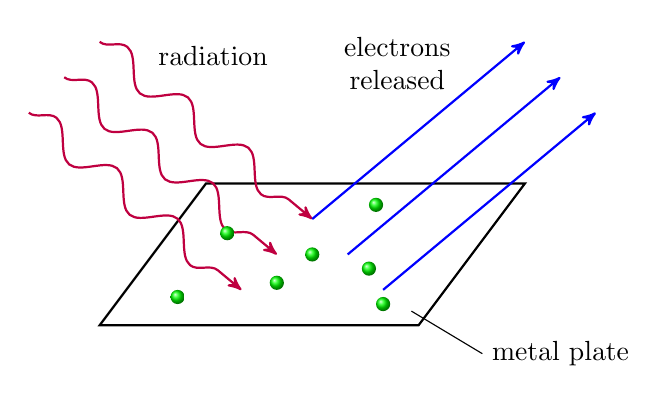
\begin{tikzpicture}[scale=0.9]
\tikzset{photon/.style={thick, decorate, purple, decoration={snake,segment length=1cm,amplitude=5pt}}}
\draw[thick] (-3,-1) -- (-1.5,1) -- (3,1) -- (1.5,-1) -- cycle;
\foreach \r in {-4,-3.5,-3} \draw[photon,->] (\r,\r+6) --++ (3,-2.5);
\foreach \r in {-0.5,0,0.5} \draw[blue,thick,->] (\r+0.5,-\r) --++ (3,2.5);
\shade [ball color = green] (0,0) circle (0.1);
\shade [ball color = green] (-1.2,0.3) circle (0.1);
\shade [ball color = green] (0.8,-0.2) circle (0.1);
\shade [ball color = green] (0.9,0.7) circle (0.1);
\shade [ball color = green] (1,-0.7) circle (0.1);
\shade [ball color = green] (-0.5,-0.4) circle (0.1);
\shade [ball color = green] (-1.9,-0.6) circle (0.1);
\draw (1.4,-0.8) --++ (1,-0.6) node[right]{metal plate};
\node at (-1.4,2.8) {radiation};
\node[twoline] at (1.2,2.7) {electrons\\released};
\end{tikzpicture}
\end{block}

\end{frame}
%----------------------------------
\begin{frame}
\tightframetitle{photoelectric effect}

\begin{block}{}
\textcolor{blue}{conduction electrons} -- not tightly held, free to move around

when EM radiation strikes metal, electrons break free
\end{block}

\pause

\begin{block}{}
this process is called \keypoint{photoelectric effect} (or photoemission)
\end{block}

\begin{block}{}
these ejected electrons are called \keypoint{photoelectrons}
\end{block}

\pause

\begin{block}{}
first observed in 1887 by \textcolor{Green}{Heinrich Hertz}, who found electrodes illuminated with ultraviolet light create electric sparks easily
\end{block}

\end{frame}

%----------------------------------
\begin{frame}
\tightframetitle{characteristic properties of photoelectric effect}

\begin{block}{}
\begin{itemize}
\item exists a minimum \keypoint{threshold frequency} $f_0$, when $f<f_0$, no electrons released

\item \textcolor{blue}{immediate} emission of electrons happens as light is turned on

\item low intensity light is effective

\item increasing \textcolor{blue}{intensity} has no effect on \textcolor{blue}{energies} of electrons

\item increasing \textcolor{blue}{intensity} of incident light increases \textcolor{blue}{number} of photoelectrons emitted

\item increasing radiation \textcolor{blue}{frequency} increases electron \textcolor{blue}{energies}
\end{itemize}
\end{block}

\end{frame}

%----------------------------------
\begin{frame}
\tightframetitle{breakdown of wave theory}

\begin{block}{}
wave theory of light fails to explain these properties
\end{block}

\begin{block}{}
according to wave model of light:
\begin{itemize}
\item greater intensity mean higher energy, easier to release electrons

\item need very intense light to have immediate effect

\item low-frequency light should work, electrons could absorb energies gradually
\end{itemize}
\end{block}

\pause

\begin{block}{}
some new ideas are here needed!
\end{block}

\end{frame}

%----------------------------------
\subsection{photon theory}
%----------------------------------
\begin{frame}
\tightframetitle{birth of quantum theory}

\begin{columns}
\column{0.7\linewidth}
\begin{block}{}
photoelectric effect was first explained by \textcolor{Green}{Albert Einstein} in 1905
\end{block}

\begin{block}{}
Albert Einstein was awarded the Nobel physics Prize in 1921 for ``\emph{his discovery of the law of the photoelectric effect}''
\end{block}

\column {0.27\linewidth}
\begin{block}{}
\centering
\includegraphics[height=100pt]{Einstein_patentoffice.jpg}
\end{block}
\end{columns}

\pause

\begin{block}{}
Einstein's revolutionary idea: light energy is \textcolor{blue}{not continuous} but carried in \textcolor{blue}{discrete packets}

all electromagnetic radiation consists of photons
\end{block}

\end{frame}

%----------------------------------
\begin{frame}
\tightframetitle{Einstein relation}

\begin{block}{}
a \keypoint{photon} is a packet (\textcolor{blue}{quanta}) of electromagnetic energy
\end{block}

\begin{block}{}
energy of one photon: $\boxed{E=hf}$ known as \keypoint{Einstein relation}

\keypoint{Planck constant}: $h=6.63\times10^{-34} \text{ J}\cdot\text{s}$
\end{block}

\pause

\begin{block2}{Example}{DarkGreen}
$\gamma$-rays are the most energetic EM waves, they have frequencies higher than $10^{20} \text{ Hz}$, estimate energy of a $\gamma$-photon:

\nskip $E=hf>6.63\times10^{-34}\times10^{20} \approx 10^{-13}\text{ J}$
\end{block2}

\end{frame}

%----------------------------------
\begin{frame}
\tightframetitle{Einstein relation: comments}

\begin{block}{}
\begin{enumerate}
\item $E \propto f$ $\Rightarrow$ higher/lower frequency, higher/lower energy

\item relate energy to wavelength: $c=\lambda f$ $\Rightarrow$ $\boxed{E=\frac{hc}{\lambda}}$

 $E \propto \frac{1}{\lambda}$ $\Rightarrow$ longer/shorter wavelength, lower/higher energy

\item Einstein relation tells connection between a particle property (energy $E$) and a wave property (frequency $f$, or wavelength $\lambda$)
\end{enumerate}
\end{block}

\end{frame}
%----------------------------------
\subsection{explanation of photoelectric effect}
%----------------------------------
\begin{frame}
\tightframetitle{explanation of photoelectric effect}

\begin{block}{}
electrons are trapped in an \textcolor{blue}{energy well} (electrostatic attraction between positive metal ions and negative electrons)
\end{block}

\begin{block}{}
an electron requires a minimum energy, called \keypoint{work function} $\Phi$, to \textcolor{blue}{escape} a metal's \textcolor{blue}{surface}
\end{block}

\begin{block}{}
an electron may \textcolor{blue}{capture} a photon and \textcolor{blue}{absorb} all its energy

if this energy is greater than $\Phi$, the electron can break free from metal
\end{block}

\end{frame}
%----------------------------------
\begin{frame}
\tightframetitle{photoelectric equation}

\begin{block}{}
\keypoint{Einstein's photoelectric equation}:
$$\boxed{hf = \Phi + E_{k,\tmax} = \Phi + \frac{1}{2}mv^2_\tmax}$$
\end{block}

\begin{block}{}
at critical condition, K.E. of emitted electron is zero
\end{block}

\begin{block}{}
threshold frequency $f_0$ is given by: $\boxed{hf_0 = \Phi}$
\end{block}

\end{frame}

%----------------------------------
\begin{frame}
\tightframetitle{further comments on photon theory}

\begin{block}{}
\begin{enumerate}
\item single photon interacts with single electron, \textcolor{blue}{one-to-one interaction} event

\item photon no longer exists after being absorbed by electron

\item greater \textcolor{blue}{intensity} means \textcolor{blue}{more photons} per unit time, so more electrons released

\item greater \textcolor{blue}{frequency} means more \textcolor{blue}{energetic} photons, so more energetic electrons

\item below threshold $f_0$, electron cannot obtain enough energy to \textcolor{blue}{overcome} $\Phi$ and hence cannot escape
\end{enumerate}
\end{block}

\end{frame}

%----------------------------------
\begin{frame}
	\tightframetitle{graphical interpretation of photoelectric equation}
	
	\begin{columns}
		\column{0.45\linewidth}
		\begin{block}{}
			\centering
			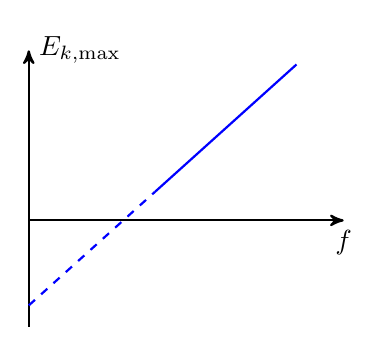
\begin{tikzpicture}[yscale=0.9]
			\draw[thick,->] (0,-1.5) -- (0,2.4) node[right]{$E_{k,\tmax}$};
			\draw[thick,->] (0,0) -- (4,0) node[below]{$f$};
			\draw[thick,blue, dashed] (0,-1.2) -- ++(1.6,1.6);
			\draw[thick,blue] (1.6,.4) -- ++(1.8,1.8);
			\end{tikzpicture}
		\end{block}
		
		\column {0.5\linewidth}
		\begin{block}{}
			rearrange equation:
			
			\nskip $ E_{k,\tmax} = hf - \Phi$
			
			plot $ E_{k,\tmax} $ against $f$, then
			
			\nskip $\text{gradient} = h$
			
			\nskip $x\text{-intercept} = \frac{\Phi}{h} = f_0$
			
			\xskip \nskip $y\text{-intercept} = -\Phi$
		\end{block}
	\end{columns}
	
	\pause
	
	\begin{block}{}
		if measurements for a set of $(f, E_{k,\tmax})$ are taken, plot a best-fit line, then Planck constant $h$, threshold frequency $f_0$, work function $\Phi$ can all be computed
	\end{block}
	
\end{frame}

%----------------------------------
\begin{frame}
\tightframetitle{electronvolt}

\begin{block}{}
define a more convenient energy unit \keypoint{electronvolt} (eV):

energy transferred when an electron travels through a potential difference of one volt

$e = 1.60\times10^{-19} \text{ C}$ $\Rightarrow$ $\boxed{1 \text{ eV} = 1.60\times10^{-19} \text{ J}}$
\end{block}

\begin{block2}{Example}{DarkGreen}
\footnotesize
Find the longest wavelength of light waves that release electrons from gold. (Work function of gold $\Phi = 4.9\text{ eV}$)

\nskip $f_0 = \frac{\Phi}{h} = \frac{4.9\times1.60\times10^{-19}}{6.63\times10^{-34}} \approx 1.18\times10^{18} \text{ Hz}$

\xskip
\nskip $\lambda_0 = \frac{c}{f_0} = \frac{3.00\times10^8}{1.18\times10^{15}} \approx 2.5\times10^{-7} \text{ m} \,$ (ultraviolet light)
\end{block2}

\end{frame}

%----------------------------------
\begin{frame}
	\tightframetitle{worked example}
	
	\begin{block2}{Why our demonstration does not work?}{DarkGreen}
		\footnotesize
		Given that the work function energy for zinc is 4.3 eV, and the wavelength of the ultraviolet torch emits is 365 nm. Explain why this wavelength does not cast any effect on the charged metal leaf of the electroscope.
	\end{block2}
	
	\pause
	
	\begin{block}{}
			
		photon energy: $E=hf=\frac{hc}{\lambda}$
		
		\nskip $\Rightarrow E = \frac{6.63\times10^{-34} \times 3.0\times10^8}{3.65\times10^{-7}} \approx 5.45\times10^{-19} \text{ J}$
			
		\xskip
		
		work function: $\Phi = 4.3 \times 1.6\times10^{-19} \approx 6.88\times10^{-19} \text{ J}$
		
		$E<\Phi$, so not enough energy to release electrons
	\end{block}
	
\end{frame}

%----------------------------------
\begin{frame}
\tightframetitle{\textcolor{orange}{summary of photoelectric effect}}

\begin{block}{}
basic principle: electron absorbs photon, acquires energy, overcomes work function, and escapes from metal surface

photoelectric equation: $hf = \Phi + \frac{1}{2}mv^2_\tmax$
\end{block}

\begin{block}{}
\centering
\begin{tabular}{|c|c|}
\hline phenomenon & explanation \\ 
\hline
\hline immediate effect & one-to-one collision event \\ 
\hline $f\nearrow$, more energetic electrons & photon energy $E\propto f$ \\ 
\hline threshold frequency & $E\propto f$ and $E>\Phi$ \\
\hline intensity $\nearrow$, more electrons & photon number $\propto$ intensity\\ 
\hline 
\end{tabular} 
\end{block}


\end{frame}



%-------------------------------
\section{wave-particlue duality}
\frame{\setstretch{.4}\Large\tableofcontents[currentsection,hideallsubsections]}
%----------------------------------
\subsection{nature of light}
%----------------------------------
\begin{frame}
	\tightframetitle{dual nature of light}
	
	\begin{block}{}
		the \textcolor{red}{dual} nature of light
		\begin{itemize}
			\item travels through \textcolor{blue}{space} as a \textcolor{blue}{wave} (electromagnetic wave) $\rightarrow$ interference, diffraction
			
			\item \textcolor{blue}{interacts} with matter as a \textcolor{blue}{particle} (photon) $\rightarrow$ photoelectric effect, emission/absorption spectrum of element, Compton scattering
		\end{itemize}
	\end{block}
	
	\pause
	
	\begin{block}{}
		\keypoint{wave-particle duality}: light shows \textcolor{blue}{both} wave-like and particle-like behaviours, it is both a wave and a particle
	\end{block}
	
\end{frame}
%----------------------------------
\subsection{matter waves}
%----------------------------------
\begin{frame}
	\tightframetitle{matter waves}
	
	\begin{block}{}
		\textcolor{Green}{Louis de Broglie} suggested in 1924 that all matter should also have a \textcolor{blue}{dual} nature
		
		de Broglie was awarded the 1929 Nobel Physics Prize ``\emph{for his discovery of the wave nature of electrons}''
	\end{block}
	
	\pause
	
	\begin{block}{}
		wave-like property can be represented by wavelength $\lambda$
		
		\keypoint{de Broglie wavelength}: $\boxed{\lambda = \frac{h}{p} = \frac{h}{mv}}$
		
		where $p=mv$ is \textcolor{blue}{momentum} of the particle
	\end{block}
	
\end{frame}
%----------------------------------
\begin{frame}
	\tightframetitle{de Broglie wavelength}
	
	\begin{block2}{Example}{DarkGreen}
		estimate de Broglie wavelength of Colin walking at $2\mps$ and electrons travelling at $10^6\mps$
	\end{block2}
	
	\pause
	
	\begin{block}{}
		\nskip $\lambda_\text{Colin} = \frac{h}{m_\text{Colin}v} = \frac{6.63 \times 10^{-34}}{60 \times 2} \approx 5.5 \times 10^{-36} \text{ m}$
		
		\nskip $\lambda_e = \frac{h}{m_\text{e}v} = \frac{6.63 \times 10^{-34}}{9.1 \times 10^{-31} \times 10^6} \approx 7.3 \times 10^{-10} \text{ m}$
		
		\xskip $\lambda_\text{Colin}$ is extremely small, so I don't look like a wave at all!
		
		but fast-moving electrons can be diffracted by solids (atomic spacing $\sim 10^{-10}\text{ m}$)
	\end{block}
	
\end{frame}
%----------------------------------
\begin{frame}
	\tightframetitle{electron diffraction}
	
	\begin{block}{}
		wave property of electron was confirmed by \textcolor{Green}{Clinton Davisson} and \textcolor{Green}{George Thomson} in 1927
	\end{block}
	
	\begin{block}{}
		they showed experimentally electrons were diffracted by metal (nickel) crystals
	\end{block}
	
	\begin{block}{}
		1937 Nobel Physics Prize was awarded jointly to Clinton Davisson and George Thomson ``\emph{for their experimental discovery of the diffraction of electrons by crystals}''
	\end{block}
	
\end{frame}
%----------------------------------
\begin{frame}
	\tightframetitle{electron diffraction experiment}
	
	\begin{block}{}
		\centering
		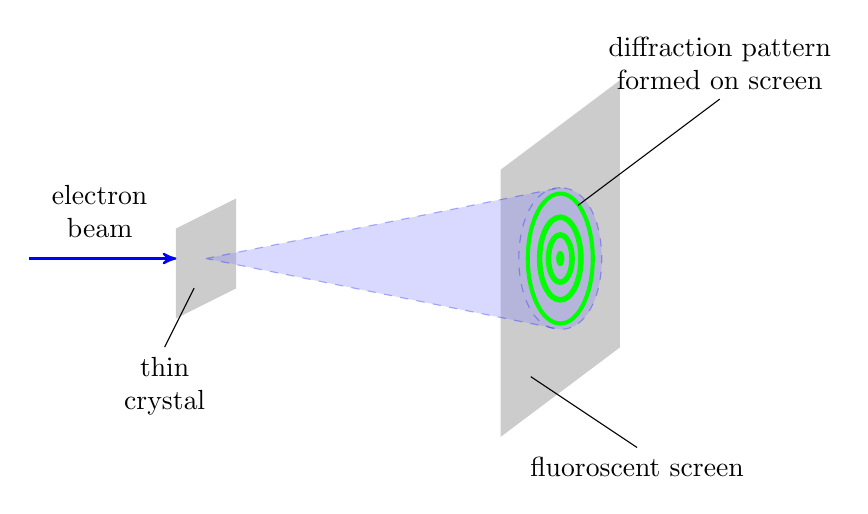
\begin{tikzpicture}[scale=0.75]
		\draw[gray!40,fill] (-0.5,-1) -- (-0.5,0.5) -- (0.5,1) -- (0.5,-0.5) -- cycle;
		\draw[thick,blue,->] (-3,0) -- (-.5,0);
		\draw[gray!40,fill] (5,-3) -- (5,1.5) -- (7,3) -- (7,-1.5) -- cycle;
		\draw[blue, dashed, fill=blue!50, opacity=0.3] (0,0) -- (6,1.2) [out = 0, in=0] to (6,-1.2) --cycle;
		\draw[blue, dashed, opacity=0.3] (6,1.2) [out = 180, in=180] to (6,-1.2);
		\draw[green,fill] (6,0) ellipse (0.06 and 0.12);
		\draw[green,line width=2pt] (6,0) ellipse (0.2 and 0.4);
		\draw[green,line width=2pt] (6,0) ellipse (0.35 and 0.7);
		\draw[green,line width=1.5pt] (6,0) ellipse (0.55 and 1.1);
		\draw (-0.2,-0.5) --++ (-0.5,-1) node[below,twoline]{thin\\crystal};
		\draw (5.5,-2) --++ (1.8,-1.2) node[below] {fluoroscent screen};
		\draw (6.3,0.9) --++ (2.4,1.8) node[above,twoline] {diffraction pattern\\formed on screen};
		\node[twoline] at (-1.8,0.8) {electron\\beam};
		\end{tikzpicture}
	\end{block}
	
\end{frame}
%----------------------------------
\begin{frame}
	\tightframetitle{electron diffraction patterns}
	
	\begin{columns}[c]
		\column{0.5\textwidth}
		\begin{block}{}
			\centering
			
			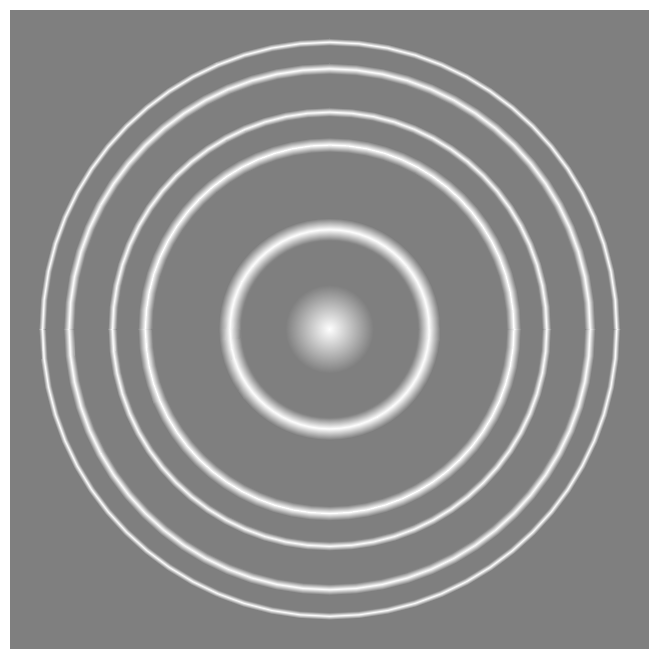
\includegraphics[height=150pt]{ring-pattern.pdf}
			
		\end{block}
		
		\column{0.5\textwidth}
		\begin{block}{}
			\centering
			\includegraphics[height=150pt]{hexagon-pattern.pdf}
		\end{block}
	\end{columns}
	
\end{frame}
%----------------------------------
\begin{frame}
	\tightframetitle{applications of electron diffraction}
	
	\begin{block}{}
		can investigate \textcolor{blue}{structure} of matter using electron diffraction
	\end{block}
	
	\begin{block}{}
		electrons of various wavelengths are used to explore arrangements of atoms, structures of complex molecules, structure of atomic nuclei, etc.
	\end{block}
	
	\begin{block}{}
		\textcolor{blue}{electron microscope}, using electrons beams with wavelengths $10^5$ shorter than visible light, better than 50 pm resolution,  magnifications up to $10^7$x
	\end{block}
	
\end{frame}

%----------------------------------
\subsection{momentum of light}
%----------------------------------

%----------------------------------
\begin{frame}
	\tightframetitle{momentum of light}
	
	\begin{block}{}
		de Broglie relation also applies to photons, this predicts a photon has momentum $\boxed{p=\frac{h}{\lambda}}$
		
		compare with Einstein relation $E=hf=\frac{hc}{\lambda}$, photon has energy spectrum $\boxed{E=pc}$
	\end{block}
	
	\pause
	
	\begin{block}{}			
		notice that this is a \textcolor{blue}{relativistic momentum}, as photons move at speed of light, definition for classical momentum $p=mv$ does not apply for photons
	\end{block}
	
\end{frame}

%----------------------------------
\begin{frame}
	\tightframetitle{example question: radiation pressure}
	
	\begin{block2}{radiation pressure on a surface}{DarkGreen}
		\small A laser of power $P=5.0$ mW incident on a spot of $A=2.0$ mm$^2$, what is the pressure caused by the beam?
	\end{block2}
	
	\pause
	
	\begin{block}{}
		\footnotesize 
		number of photons incident in $\Delta t$ is:
		
		\nskip $\Delta N = \frac{\text{total energy of beam}}{\text{energy of each photon}} = \frac{P\Delta t}{hf}$
		
		each photon exerts a force:
		
		\nskip $F_0 = \frac{\text{change in momentum}}{\text{time taken}} = \frac{\Delta p}{\Delta t} = \frac{h}{\lambda \Delta t}$
		
		pressure caused by laser beam:
		
		\nskip $p = \frac{F}{A} = \frac{\Delta N \times F_0}{A} = \frac{P\Delta t}{hf} \times \frac{h}{\lambda \Delta t} \times \frac{1}{A}$ $\,\Rightarrow\,$ $p= \frac{P}{cA}$
		
		\nskip $p=\frac{5.0\times10^{-3}}{3.0\times10^8 \times 2.0\times10^{-6}} = 8.3 \times 10^{-6} \text{ Pa}$
	\end{block}
	
\end{frame}


%----------------------------------
\subsection{wave-particle duality}
%----------------------------------


%----------------------------------
\begin{frame}
	\tightframetitle{wave-particle duality}
	
	
	\begin{block}{electromagnetic radiation}
		\begin{itemize}
			\item particle-like behaviour: photoelectric effect, radiation pressure
			
			\item wave-like behaviour: interference, diffraction, Doppler effect, reflection \& refraction
		\end{itemize}
	\end{block}

\begin{block}{matter particles}
	\begin{itemize}
		\item particle-like behaviour: deflection in electric/magnetic fields, decay, scattering
		
		\item wave-like behaviour: electron diffraction
	\end{itemize}
\end{block}
	
\end{frame}



%----------------------------------
\begin{frame}
	\tightframetitle{wave-particle duality and beyond}
	
	\begin{block}{}
		everything has a universal \keypoint{dual} nature
			
		light/electron/atom/bird/earth ... both a wave and a particle $\Rightarrow$ \keypoint{wave-particle duality}
	\end{block}
		
	\begin{block}{}
		wave-particle duality addresses breakdown of classical concepts like `particle' or `wave'
		
		to fully describe the behaviour of microscopic objects, need rewrite theory of classical mechanics $\longrightarrow$ \keypoint{quantum mechanics}
	\end{block}
	
	
	\begin{block}{}
		\emph{``The nature is not only queerer than we suppose, but queerer than we can suppose.''}
		--- \textcolor{Green}{J.B.S. Haldane}, Possible Worlds
	\end{block}
	
\end{frame}



%-------------------------------
\section{quantisation of energy levels}
\frame{\setstretch{.4}\Large\tableofcontents[currentsection,hideallsubsections]}
%----------------------------------


%----------------------------------
\subsection{energy levels}
%----------------------------------
\begin{frame}
	\tightframetitle{quantised energy states}
	
	
	\begin{columns}[c]
		\column{0.5\textwidth}
		\begin{block}{}
			\begin{center}
				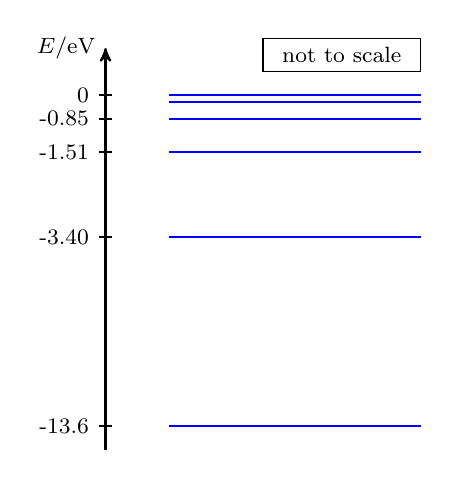
\begin{tikzpicture}[yscale=0.6,xscale=0.8]
				\foreach \s in {7,3,1.2,0.5,0.15,0}
				\draw[thick,blue] (0,-\s) -- ++ (4,0);
				\draw[thick] (-0.9,-7) -- (-1.1,-7) node[left]{\footnotesize{-13.6}};
				\draw[thick] (-0.9,-3) -- (-1.1,-3) node[left]{\footnotesize{-3.40}};
				\draw[thick] (-0.9,-1.2) -- (-1.1,-1.2) node[left]{\footnotesize{-1.51}};
				\draw[thick] (-0.9,-0.5) -- (-1.1,-0.5) node[left]{\footnotesize{-0.85}};
				\draw[thick] (-0.9,0) -- (-1.1,0) node[left]{\footnotesize{0}};
				\draw[thick,->] (-1,-7.5) -- (-1,1) node[left]{\footnotesize{$E$/\text{eV}}};
				\draw (1.5,0.5) rectangle node{\footnotesize{not to scal}e} (4,1.2);
				\end{tikzpicture}
				
				\footnotesize energy levels of a hydrogen atom
			\end{center}
		\end{block}
		
		\pause
		
		\column{0.5\textwidth}
		\begin{block}{}
			electrons in an atom only take certain orbits, corresponding to certain \textcolor{blue}{fixed} values of energy
		\end{block}
		
		\begin{block}{}
			energy of electrons in an atom is \keypoint{discrete}/\keypoint{quantised}, called \keypoint{energy levels}

		\end{block}
	\end{columns}
	
\end{frame}

%----------------------------------
\begin{frame}
	\tightframetitle{comments on energy level}
	
	\begin{block}{}
		\begin{enumerate}
			\item energy levels are always \textcolor{blue}{negative} 
			
			external energy needed to remove electrons from an atom
			
			\item an electron with \textcolor{blue}{zero} energy is a \textcolor{blue}{free} electron
			
			\item meaning of \textcolor{blue}{quantisation}
			
			an electron can have only one of these values of energy
			
			cannot have an energy between energy levels
			
			e.g., only $E_1$, $E_2$, $E_3$, but no intermediate values
		\end{enumerate}
	\end{block}
	
\end{frame}

%----------------------------------
\begin{frame}
	\tightframetitle{Bohr's theory of hydrogen atom}
	
	\begin{columns}
		\column{0.7\linewidth}
		\begin{block}{}
			theoretical explanation for energy levels was developed in 1913 by Danish physicist \textcolor{Green}{Niels Bohr} in his theory of \textcolor{blue}{hydrogen atom}
		\end{block}
		
		\begin{block}{}
			Neils Bohr received the Nobel Physics Prize in 1922 ``\emph{for his services in the investigation of the structure of atoms and of the radiation emanating from them}''
		\end{block}
		
		\column{0.3\linewidth}
		\begin{block}{}
			\centering
			\includegraphics[height=128pt]{Niels_Bohr.jpg}
		\end{block}
	\end{columns}
	
	
\end{frame}

%----------------------------------
\begin{frame}
	\tightframetitle{electron transitions}
	
	\begin{block}{}
		an electron can \textcolor{blue}{jump} between energy levels $\longrightarrow$ \keypoint{transitions}
	\end{block}
	
	\pause
	
	\begin{block}{}
		transition to lower level $\rightarrow$ \textcolor{blue}{lose} energy $\rightarrow$ \textcolor{blue}{emit} photon
		
		transition to higher level $\rightarrow$ \textcolor{blue}{require} energy $\rightarrow$ \textcolor{blue}{absorb} photon with the correct energy
	\end{block}
	
	\pause
	
	\begin{block}{}
		quantised energy levels $\Rightarrow$ only \textcolor{blue}{certain wavelengths} permitted
		
		this gives rise to \textcolor{blue}{discrete} emission/absorption line spectra
	\end{block}
	
\end{frame}
%----------------------------------
\begin{frame}
	\tightframetitle{emission/absorption of photons}
	
	\begin{columns}[c]
		\column{0.5\textwidth}
		\begin{block}{}
			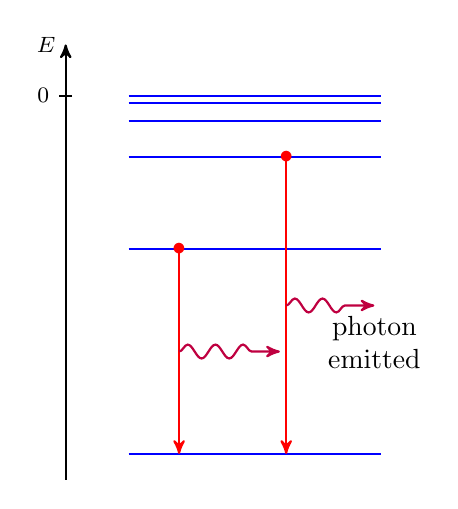
\begin{tikzpicture}[yscale=0.65,xscale=0.8]
			\foreach \s in {7,3,1.2,0.5,0.15,0}
			\draw[thick,blue] (0,-\s) -- ++ (4,0);
			\draw[thick] (-0.9,0) -- (-1.1,0) node[left]{\footnotesize{0}};
			\draw[thick,->] (-1,-7.5) -- (-1,1) node[left]{\footnotesize{$E$}};
			\draw[red,thick,->] (0.8,-3) node{$\bullet$} -- (0.8,-7);
			\draw[red,thick,->] (2.5,-1.2) node{$\bullet$} -- (2.5,-7);
			\draw [->, thick, purple, decorate, decoration={snake,post=lineto, post length=2mm}] (0.8,-5) -- (2.4,-5) ;
			\draw [->, thick, purple, decorate, decoration={snake,post=lineto, post length=2mm}] (2.5,-4.1) -- (3.9,-4.1) node[below,align=center,execute at begin node=\setlength{\baselineskip}{1.2em}]{\textcolor{black}{photon}\\\textcolor{black}{emitted}};
			\end{tikzpicture}
		\end{block}
		
		\column{0.5\textwidth}
		\begin{block}{}
			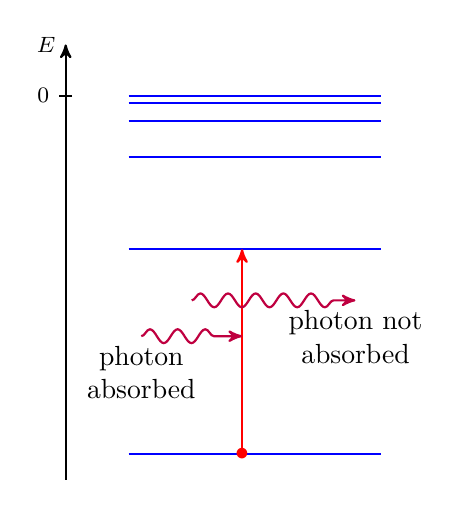
\begin{tikzpicture}[yscale=0.65,xscale=0.8]
			\foreach \s in {7,3,1.2,0.5,0.15,0}
			\draw[thick,blue] (0,-\s) -- ++ (4,0);
			\draw[thick] (-0.9,0) -- (-1.1,0) node[left]{\footnotesize{0}};
			\draw[thick,->] (-1,-7.5) -- (-1,1) node[left]{\footnotesize{$E$}};
			\draw[red,thick,<-] (1.8,-3) -- (1.8,-7) node{$\bullet$};
			\draw [->, thick, purple, decorate, decoration={snake,post=lineto, post length=2mm}] (0.2,-4.7) node[below,align=center,execute at begin node=\setlength{\baselineskip}{1.2em}]{\textcolor{black}{photon}\\\textcolor{black}{absorbed}} -- (1.8,-4.7) ;
			\draw [->, thick, purple, decorate, decoration={snake,post=lineto, post length=2mm}] (1,-4) -- (3.6,-4) node[below,align=center,execute at begin node=\setlength{\baselineskip}{1.2em}]{\textcolor{black}{photon not}\\\textcolor{black}{absorbed}};
			\end{tikzpicture}
		\end{block}
	\end{columns}
	
\end{frame}


%----------------------------------
\subsection{line spectra}

%----------------------------------
\begin{frame}
	\tightframetitle{discrete spectrum: emission spectrum}
	
	\begin{block}{}
		\textcolor{blue}{hot gas} of an element gives a unique collection of \textcolor{blue}{sharp} and \textcolor{blue}{bright lines} seen in the spectrum $\longrightarrow$ \keypoint{emission line spectrum}
	\end{block}
	
	\begin{block}{}
		emission spectrum is a \keypoint{discrete spectrum}
	\end{block}
	
	\begin{block}{}
		emission spectrum can be used to identify \textcolor{blue}{elements}
	\end{block}
	
	\begin{block}{}
		\centering
		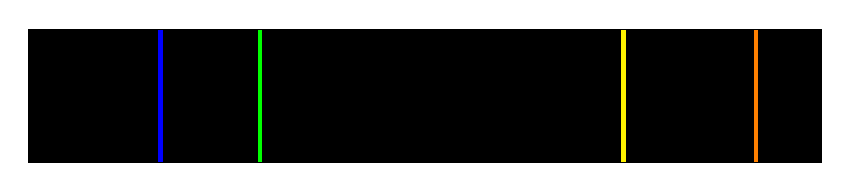
\begin{tikzpicture}[scale=0.84]
		\draw [fill] (0,0) rectangle (12,2);
		\draw [ultra thick, orange] (11,0) -- (11,2);
		\draw [ultra thick, yellow] (9,0) -- (9,2);
		\draw [ultra thick, green] (3.5,0) -- (3.5,2);
		\draw [ultra thick, blue] (2,0) -- (2,2);
		\end{tikzpicture}
	\end{block}
	
\end{frame}

%----------------------------------
\begin{frame}
	\tightframetitle{explanation of emission spectrum}
	
	\begin{block}{}
		electrons \textcolor{blue}{excited} to higher energy states by fast-moving free electrons (accelerated by high voltage)
	\end{block}
	
	\pause
	
	\begin{block}{}
		when excited electrons return to \textcolor{blue}{ground states}, they \textcolor{blue}{emit} photons of certain frequencies 
	\end{block}
	
	\pause
	
	\begin{block}{}
		each frequency corresponds to a line in \textcolor{blue}{emission spectrum}
	\end{block}
	
\end{frame}

%----------------------------------
\begin{frame}
	\tightframetitle{example question: transition of electrons}
	
	\begin{block2}{transition of electrons}{DarkGreen}
		An electron falls from the second level (-3.40 eV) to lowest energy level (\keypoint{ground state}\index{ground state}) (-13.6 eV) of a hydrogen atom. Find the wavelength of the light emitted.
	\end{block2}
	
	\pause
	
	\begin{block}{}
		\nskip $hf = \Delta E$ $\Rightarrow$ $f = \frac{E_2-E_1}{h}$
		
		\xskip \nskip $f = \frac{(-3.40\text{ eV})-(-13.6\text{ eV})}{6.63\times 10^{-34} \text{ J}\cdot\text{s}} \approx 2.46\times 10^{15}\text{ Hz}$
		
		\xskip \nskip $\lambda = \frac{c}{f} = \frac{3.00\times 10^8}{2.46\times 10^{15}} \approx 1.22\times 10^{-7}\text{ m}$ (ultraviolet band)
	\end{block}
	
\end{frame}

%----------------------------------
\begin{frame}
	\tightframetitle{example question: hydrogen spectrum}
	
	\begin{block2}{Hydrogen spectrum}{DarkGreen}
		\small
		Neutral hydrogen atoms are excited to the third level. The atoms then de-excite, emitting light until settling to the ground state.
		
		How many emission lines are observed?
		
		Which transition gives out emission line with shortest wavelength?
	\end{block2}
	
	\pause
	
	\begin{block}{}
		possible transitions: $E_3 \to E_2$, $E_2 \to E_1$, $E_3 \to E_1$
		
		so a total of 3 emission lines
	\end{block}
	
	\pause
	
	\begin{block}{}
		$\frac{hc}{\lambda} = \Delta E$, smallest $\lambda$ so greatest $\Delta E$, this corresponds to the transition $E_3 \to E_1$
	\end{block}
	
\end{frame}

%----------------------------------
\begin{frame}
	\tightframetitle{fluorescent tubes ($\star$)}
	
	\begin{block}{}
		\keypoint{fluorescent tubes} contain \textcolor{blue}{mercury vapour}, across which a high voltage is applied, electrons are excited and then return to ground states, emitting photons in \textcolor{blue}{UV} range
	\end{block}
	
	\begin{block}{}
		a \textcolor{blue}{fluorescent material} (e.g., a phosphorus coating) on inside of tube absorbs these photons, exciting its electrons to much higher states, these electrons then \textcolor{blue}{cascade} down the energy levels, emitting many photons in the form of \textcolor{blue}{visible} light
	\end{block}
	
\end{frame}


%----------------------------------
\begin{frame}
\tightframetitle{continuous spectrum}

\begin{block}{}
splitting light (with a \textcolor{blue}{prism}, \textcolor{blue}{diffraction grating}, etc.) into its different wavelengths, this process is called \keypoint{dispersion} of light, this gives a \keypoint{spectrum}
\end{block}

\begin{block}{}
\textcolor{blue}{white} light (eg. sunlight) consists of a range of wavelengths or frequencies $\longrightarrow$ giving a \keypoint{continuous spectrum}
\end{block}

\begin{block}{}
\centering
\pgfdeclareverticalshading{rainbow}{100bp}
{color(0bp)=(Red); color(25bp)=(Red); color(30bp)=(OrangeRed); color(35bp)=(Orange); color(40bp)=(Gold); color(45bp)=(Yellow); color(50bp)=(GreenYellow); color(55bp)=(LimeGreen); color(60bp)=(Teal); color(65bp)=(DarkBlue); color(70bp)=(Indigo); color(75bp)=(Purple); color(100bp)=(Purple)}
\begin{tikzpicture}[shading=rainbow]
\shade[shading angle=90] (0,0) rectangle (10,2);
\end{tikzpicture}
\end{block}

\end{frame}


%----------------------------------
\begin{frame}
\tightframetitle{discrete spectrum: absorption spectrum}

\begin{block}{}
pass white light through a \textcolor{blue}{cool gas}, certain wavelengths are \textcolor{blue}{missing}, \textcolor{blue}{dark lines} appear in background of continuous spectrum $\longrightarrow$ \keypoint{absorption line spectrum}
\end{block}

\begin{block}{}
absorption spectrum is a \keypoint{discrete spectrum}
\end{block}

\begin{block}{}
absorption spectrum is used to study components of stars
\end{block}

\begin{block}{}
\centering
\begin{tikzpicture}[shading=rainbow,scale=0.84]
\shade[shading angle=90] (0,0) rectangle (12,2);
\foreach \x  in {1.9,4.4,5.9,7.6,8.2,9.9,11.4}
\draw [very thick] (\x,0) -- (\x,2);
\end{tikzpicture}
\end{block}

\end{frame}


%----------------------------------
\begin{frame}
\tightframetitle{explanation of absorption spectrum}

\begin{block}{}
at low temperatures, most electrons stay in \textcolor{blue}{ground states}
\end{block}

\pause

\begin{block}{}
pass a light through cold gas, photons of correct wavelength are \textcolor{blue}{absorbed} by electrons to excite them to higher energy levels
\end{block}

\pause

\begin{block}{}
these wavelengths are then missing, corresponding to lines in \textcolor{blue}{absorption spectrum}
\end{block}

\end{frame}

%----------------------------------
\begin{frame}
\tightframetitle{transition and photon emission/absorption}

\begin{block}{}
\textcolor{blue}{energy} of photon to be emitted/absorbed must \textcolor{blue}{match} the gap between two energy levels
\end{block}

\begin{block}{}

energy \textcolor{blue}{conserved} during electron and photon interaction 
\end{block}

\pause

\begin{block}{}
\centering $\boxed{hf = \Delta E} \quad$ (for both emission/absorption processes)
\end{block}

\end{frame}

%----------------------------------
\begin{frame}
	\tightframetitle{example question: counting dark lines}
	
	\begin{block2}{}{DarkGreen}
		\small A white light of wavelengths $420\sim740$ nm passes through a cool gas cloud. Electron energy levels of gas atoms are: $E_1=-13.6$ eV, $E_2=-3.41$ eV, $E_3=-1.50$ eV, and $E_4=-0.85$ eV.
		
		How many dark lines can be seen in the emergent spectrum?
	\end{block2}
	
	\pause
	
	\begin{block}{}
		\small use $E=\frac{hc}{\lambda}$ to find range of photon energies: $1.68\sim2.96$ eV
	\end{block}
	
	\pause
	
	\begin{block}{}
		\small possible absorptions: $E_2 \to E_3 \,(1.91\text{ eV})$, $E_2 \to E_4 \,(2.56\text{ eV})$
		
		so two dark lines in the absorption spectrum
	\end{block}
	
\end{frame}



%----------------------------------
\begin{frame}
	\tightframetitle{\textcolor{orange}{summary of energy levels}}
	
	\begin{block}{}
		\textcolor{blue}{electrons} can only take \textcolor{blue}{discrete} energy levels
		
		when electrons make \textcolor{blue}{transitions} from one level to another, energy is released or absorbed
		
		this is related to emission or absorption of \textcolor{blue}{photon} with the correct \textcolor{blue}{frequency}
	\end{block}
	
	\begin{block}{}		
		\textcolor{blue}{quantised} energy levels for electrons, so only photons or certain \textcolor{blue}{wavelengths} are emitted or absorbed		
	\end{block}
	
\end{frame}

%-------------------------------
\section{band theory}
\frame{\setstretch{.4}\Large\tableofcontents[currentsection,hideallsubsections]}
%----------------------------------
\subsection{energy bands}
%----------------------------------

%----------------------------------
\begin{frame}
	\tightframetitle{energy bands}
	
	\begin{block}{}
		in an isolated atom, electrons have discrete energy levels 
	
	\end{block}
	
	\begin{block}{}
		in solids, interaction between neighbouring atoms causes change in configuration of energies

		original energy levels split into a band with many \textcolor{blue}{sub-levels}
	\end{block}
	
	\begin{block}{}
		number of sub-levels in each band equals number of atoms in solid
		
		very large number of atoms present, so sub-levels (seem to) form \textcolor{blue}{continuous} \textcolor{red}{energy bands}
	\end{block}
	
\end{frame}

%----------------------------------
\begin{frame}
	\tightframetitle{energy bands}
	
	\begin{block}{}
		\centering
		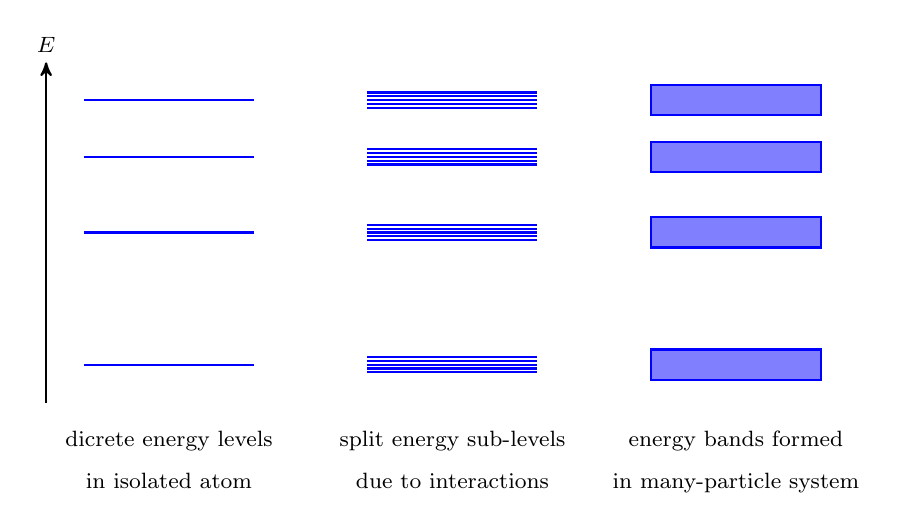
\begin{tikzpicture}[yscale=0.48,xscale=.6]
		\foreach \s in {0,1.5,3.5,7}{
			\draw[thick,blue] (0,-\s) -- ++ (3.6,0);
			\draw[thick,blue] (6,-\s) -- ++ (3.6,0) (6,-\s+0.1) -- ++ (3.6,0) (6,-\s-0.1) -- ++ (3.6,0) (6,-\s+0.2) -- ++ (3.6,0) (6,-\s-0.2) -- ++ (3.6,0);
			\draw[thick,blue,fill=blue!50] (12,-\s-0.4) rectangle (15.6,-\s+0.4);
		}
		\draw[thick,->] (-.8,-8) -- (-.8,1) node[above]{{\footnotesize $E$}};
		\node[below,align=center,execute at begin node=\setlength{\baselineskip}{1.5em}] at (1.8,-8.5) {{\footnotesize dicrete energy levels}\\{\footnotesize in isolated atom}};
		\node[below,align=center,execute at begin node=\setlength{\baselineskip}{1.5em}] at (7.8,-8.5) {{\footnotesize split energy sub-levels}\\{\footnotesize due to interactions}};
		\node[below,align=center,execute at begin node=\setlength{\baselineskip}{1.5em}] at (13.8,-8.5) {{\footnotesize energy bands formed}\\{\footnotesize in many-particle system}};
		\end{tikzpicture}
	\end{block}
	
\end{frame}

%----------------------------------
\begin{frame}
	\tightframetitle{band structure}
	
	\begin{block}{}
		\textcolor{red}{forbidden bands} represent energies that electrons are not allowed to take
	\end{block}
	
	\begin{block}{}		
		electrons fill up from lowest energy bands available
		
		highest fully filled band is called \textcolor{red}{valence band}
		
		next partially filled or empty band is called \textcolor{red}{conduction band}
	\end{block}
	
	\begin{block}{}		
		energy separation between valence band and conduction band defines \textcolor{red}{energy gap} of material
	\end{block}
	
\end{frame}

%----------------------------------
\begin{frame}
	\tightframetitle{band structure}
	
	\begin{block}{}
		\centering
		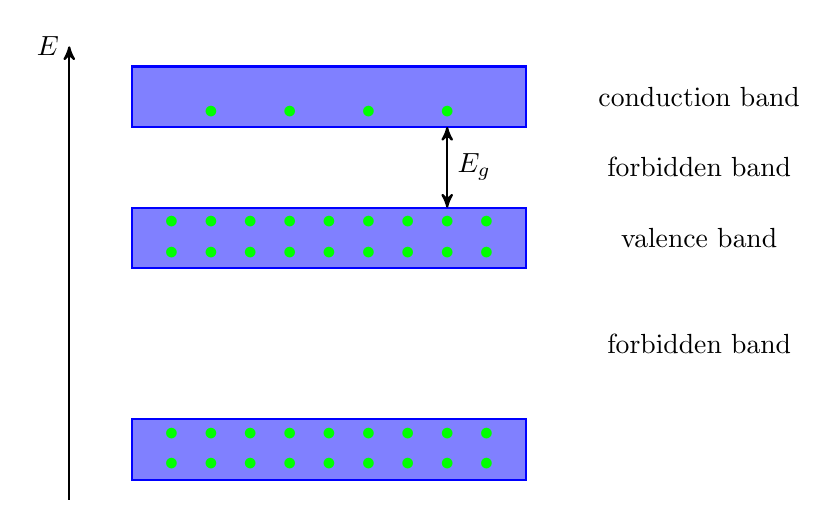
\begin{tikzpicture}[yscale=.64]
		\draw[thick,->] (-.8,-8) -- (-.8,1) node[left]{$E$};
		\foreach \s in {0,2.8,7}
		\draw[thick,blue,fill=blue!50] (0,-\s-0.6) rectangle (5,-\s+0.6);
		\foreach \x in {0.5,1,...,4.5} \foreach \y in {7.3,6.7,2.5,3.1}
		\node at (\x,-\y) {\textcolor{green}{$\bullet$}};
		\foreach \x in {1,2,3,4}
		\node at (\x,-0.3) {\textcolor{green}{$\bullet$}};
		\node at (7.2,0) {conduction band};
		\node at (7.2,-1.4) {forbidden band};
		\node at (7.2,-2.8) {valence band};
		\node at (7.2,-4.9) {forbidden band};
		\draw[thick,<->] (4,-0.6) -- (4,-2.2) node[midway,right]{$E_g$};
		\end{tikzpicture}
	\end{block}
	
\end{frame}

%----------------------------------
\subsection{band theory \& electrical conductivity}
%----------------------------------

%----------------------------------
\begin{frame}
	\tightframetitle{band theory \& electrical conductivity}
	
	\begin{block}{}
		\textcolor{blue}{electrical conductivity} of material can be explained by its band structure
	\end{block}
	
	\begin{block}{}		
		energy bands up to valence band in a solid are \textcolor{blue}{fully filled}, all states available are occupied, these electrons cannot move freely to form electric currents
		
		so the number of \textcolor{blue}{free electrons} available in \textcolor{blue}{conduction band} is the key to electrical conductivity
	\end{block}
	
\end{frame}



%----------------------------------
\begin{frame}
	\tightframetitle{insulators}
	
	\begin{block}{}
		\textcolor{blue}{conduction band} of an insulator is \textcolor{blue}{empty}
		
		\textcolor{blue}{valence band} is \textcolor{blue}{fully filled}
		
		so no movement of electron is possible
	\end{block}
	
	\begin{block}{}			
		insulators also have \textcolor{blue}{large energy gaps} $E_g$, so thermal or photo-excitation cannot easily make valence electrons jump into conduction band
		
		so insulators are \textcolor{blue}{poor conductors} of electric currents
	\end{block}
	
\end{frame}

%----------------------------------
\begin{frame}
	\tightframetitle{semi-conductors}
	
	\begin{block}{}
		band structure of semi-conductors is similar to insulators: an empty conduction band and a fully-filled valence band
		
		but semi-conductors have much \textcolor{blue}{narrower gaps}
	\end{block}
	
	\begin{block}{}			
		as \textcolor{blue}{temperature} rises, valence electrons gain thermal energy, these \textcolor{blue}{excited} electrons \textcolor{blue}{cross} the energy gap and enter conduction band
	\end{block}
	
\end{frame}

%----------------------------------
\begin{frame}
	\tightframetitle{charge carriers in semi-conductors}
	
	\begin{block}{}
		electrons entering conduction band become free electrons that can flow through material
		
		at the same time, \textcolor{red}{holes}\footnote{\textcolor{gray}{A hole has a positive charge, since an electron is missing from its site. Neighbouring electrons can move to fill the hole and leave a new hole, but this can be thought of as the hole moves about.}} are formed in valence band
	\end{block}
	
	\begin{block}{}			
		there are \textcolor{blue}{negative (electrons)} as well as \textcolor{blue}{positive (holes)} \textcolor{red}{charge carriers} in semi-conductors
		
		more charge carriers available, this contributes to conductivity
	\end{block}

\end{frame}

%----------------------------------
\begin{frame}
	\tightframetitle{charge carriers in semi-conductors}
	
	\begin{block}{}
		\textcolor{blue}{lattice vibration} would also increase at higher temperature
		
		this causes greater scattering of charge carriers
	\end{block}
	
	\begin{block}{}			
		effect of more charge carriers is far greater than lattice vibration, so \textcolor{blue}{resistance decreases} with temperature
	\end{block}

	\begin{block}{}			
		now you understand why \textcolor{blue}{thermistors} have lower resistance at higher temperature
	\end{block}
\end{frame}



%----------------------------------
\begin{frame}
	\tightframetitle{example question: energy gap calculations}
	
	\begin{block2}{good conductor or bad conductor?}{DarkGreen}
		Diamond and silicon, have energy gap $E_g \approx 6.0 \text{ eV}$ and $1.1 \text{ eV}$ respectively, argue whether they conducting when exposed to red light of $600 \text{ nm}$.
	\end{block2}
	
	\pause
	
	\begin{block}{}
		{\small energy of radiation:}
		
		\nskip {\footnotesize $E=\frac{hc}{\lambda} = \frac{6.63\times10^{-34}\times3.0\times10^8}{600\times10^{-9}} \approx 3.32\times10^{-19} \text{ J} \approx 2.1 \text{ eV}$}
		
		{\small sufficient to make valence electrons in silicon to cross energy gap, so silicon becomes conducting
		
		but not enough to excite valence electrons in diamond, so diamond remains insulator and transparent to red light}
		
	\end{block}
	
\end{frame}

%----------------------------------
\begin{frame}
	\tightframetitle{metallic conductors}
	
	\begin{block}{}
		\textcolor{blue}{conduction band} of typical metal \textcolor{blue}{overlaps} with \textcolor{blue}{valence band}
		
		no band gap means there are vacant states for conduction electrons to occupy at ease
		
		this means \textcolor{blue}{conduction electrons} are \textcolor{blue}{free} to move around to form currents, so metals are good conductors
	\end{block}
	
	\begin{block}{}
		as temperature rises, almost no change in number of conduction electrons, but \textcolor{blue}{lattice vibration} increases, electrons are more likely to be \textcolor{blue}{scattered}, so resistance would increase
	\end{block}
	
\end{frame}

%----------------------------------
\begin{frame}
	\tightframetitle{comments on conductors}
	
	\begin{block}{}
		\footnotesize
		\begin{itemize}
			\item metals are \textcolor{blue}{opaque} to visible light or other \textcolor{blue}{low-frequency} radiation
			
			width of conduction band for typical metal is about $2\sim3 \text{ eV}$
			
			low-energy photons can be absorbed by conduction electrons
			
			\item metals are \textcolor{blue}{transparent} to \textcolor{blue}{high-frequency} radiation such as X-rays
			
			if X-ray photons are absorbed, electrons would enter forbidden band
			
			but this is not allowed, so high-frequency photons penetrate through
			
			\item as conduction electrons flow, they dissipate energy as \textcolor{blue}{heat}
			
			they give off kinetic energy as they get \textcolor{blue}{scattered} by metal ions
			
			\textcolor{blue}{thermal vibration} of metal lattice increases, causing heating effects
		\end{itemize}
	\end{block}
	
\end{frame}

%----------------------------------
\begin{frame}
\tightframetitle{\textcolor{orange}{summary of band theory}}

\begin{block}{}		
	for thermistor/LDR, VB is fully filled, CB is empty
	
	as $T$/light intensity $\nearrow$, VB electrons absorb energy
	
	they cross band gap and enter CB
	
	free electrons become available in CB, holes are formed in VB
	
	more charge carriers available, so resistance decreases
\end{block}

\begin{block}{}
	for metallic conductors, CB and VB overlap (no band gap)
	
	as $T\nearrow$, no change in number of free electrons
	
	but greater thermal vibration
	
	so resistance of metal increases
\end{block}

\end{frame}


%---------------------------------
\end{document} 
